\documentclass[12pt, twoside, a4paper]{report}
\pagestyle{headings}
\pagestyle{empty}
\usepackage{indentfirst}
\usepackage{graphicx}
\usepackage[english, greek]{babel} % mine
\usepackage[utf8x]{inputenc}  % mine
\usepackage{makeidx}  % mine
\usepackage[nottoc]{tocbibind}  % mine
\usepackage{babelbib}  % mine
\makeindex  % mine

\begin{document}
\selectlanguage{greek} % mine

\title{
\vspace{-6ex}
\begin{center}

\includegraphics[scale=1]{pyrforos.png}  % mine -- no .eps files with pdflatex
\end{center}
\Large{Ε}\large{ΘΝΙΚΟ}
\Large{Μ}\large{ΕΤΣΟΒΙΟ}
\Large{Π}\large{ΟΛΥΤΕΧΝΕΙΟ} \\
\normalsize{Τ}\small{ΜΗΜΑ}
\normalsize{Η}\small{ΛΕΚΤΡΟΛΟΓΩΝ}
\normalsize{Μ}\small{ΗΧΑΝΙΚΩΝ}
\normalsize{Κ}\small{ΑΙ}
\normalsize{Μ}\small{ΗΧΑΝΙΚΩΝ}
\normalsize{Υ}\small{ΠΟΛΟΓΙΣΤΩΝ} \\
\vspace{2ex}
-ΕΙΣΑΓΕΤΕ ΤΟΝ ΤΟΜΕΑ- \\
-ΕΙΣΑΓΕΤΕ ΤΟ ΕΡΓΑΣΤΗΡΙΟ- \\
\vspace{8ex}
\large \textbf{-Εισάγετε τον τίτλο της διπλωματικής εργασίας-} \\
\vspace{10ex}
\large
ΔΙΠΛΩΜΑΤΙΚΗ ΕΡΓΑΣΙΑ \\
\vspace{2ex}
\normalsize
-Εισάγετε το σωστό άρθρο (της/του/των)- \\
\vspace{2ex}
\parbox[c]{0.4\textwidth} { \center\textbf{
-Εισάγετε το όνομα, αρχικό πατρώνυμου και επωνυμο των συγγραφέων- }}
\selectlanguage{english}  % mine -- to make sense
\parbox[c]{0.4\textwidth} { \center\textbf{
	-another author, whose name is here- }}
\selectlanguage{greek}  % mine again
\vspace{10ex}
\flushleft
\begin{tabbing}
	\textbf{Επιβλέπων}: \= -Εισάγετε το όνομα, αρχικό πατρωνύμου
				και επίθετο- \\
			    \> -Εισάγετε τον τίτλο του επιβλέποντα-
\end{tabbing}
}
\date{
\normalsize
Αθήνα, -Εισάγετε το μήνα και το έτος κατάθεσης της εργασίας-}

\maketitle
\newpage
\hspace{10pt}
%\tiny
%(this page is left intentionally blanc)
%\normalsize
% \newpage

\includegraphics{pyrforos.png}  % mine -- no .eps files with pdflatex
\noindent
\parbox[b]{0.6\textwidth} {\textbf{
\noindent
\normalsize{Ε}\small{ΘΝΙΚΟ}  % mine -- this needs modification
\normalsize{Μ}\small{ΕΤΣΟΒΙΟ}
\normalsize{Π}\small{ΟΛΥΤΕΧΝΕΙΟ}} \\
\small
ΤΜΗΜΑ ΗΛΕΚΤΡΟΛΟΓΩΝ ΜΗΧΑΝΙΚΩΝ ΚΑΙ ΜΗΧΑΝΙΚΩΝ ΥΠΟΛΟΓΙΣΤΩΝ \\
-ΕΙΣΑΓΕΤΕ ΤΟΝ ΤΟΜΕΑ- \\
-ΕΙΣΑΓΕΤΕ ΤΟ ΕΡΓΑΣΤΗΡΙΟ-}

\begin{center}
\vspace{8ex}
\large \textbf{-Εισάγετε τον τίτλο της διπλωματικής εργασίας-} \\
\vspace{10ex}
\large
ΔΙΠΛΩΜΑΤΙΚΗ ΕΡΓΑΣΙΑ \\
\vspace{2ex}
\normalsize
-Εισάγετε το σωστό άρθρο (της/του/των)- \\
\vspace{2ex}
\parbox[c]{0.4\textwidth} { \center\textbf{
-Εισάγετε το όνομα, αρχικό πατρώνυμου και επωνυμο των συγγραφέων- }}
\selectlanguage{english}  % mine -- to make sense
\parbox[c]{0.4\textwidth} { \center\textbf{
	-another author, whose name is here- }}
\selectlanguage{greek}  % mine again
\vspace{10ex}
\flushleft
\begin{tabbing}
\textbf{Επιβλέπων}: \= -Εισάγετε το όνομα, αρχικό πατρωνύμου
			και επίθετο- \\
		    \> -Εισάγετε τον τίτλο του επιβλέποντα-
\end{tabbing}
\end{center}

\noindent
Εγκρίθηκε από την τριμελή εξεταστική επιτροπή την -εισάγετε ημερομηνία-.

\begin{center}
\scriptsize
\parbox[b]{0.3\textwidth} {\center
	........................................
	-Εισάγετε ονοματεπώνυμο-
	-Εισάγετε τίτλο-
}
\parbox[b]{0.3\textwidth} {\center
	........................................
	-Εισάγετε ονοματεπώνυμο-
	-Εισάγετε τίτλο-
}
\parbox[b]{0.3\textwidth} {\center
	........................................
	-Εισάγετε ονοματεπώνυμο-
	-Εισάγετε τίτλο-
}
\end{center}
\vspace{10ex}
\normalsize
\noindent
Αθήνα, (εισάγετε το μήνα και το έτος κατάθεσης της εργασίας).
\newpage
\hspace{10pt}

\vspace{30ex}
\noindent
................................... \\
\textbf{(Εισάγετε όνομα, αρχικό πατώνυμου και επίθετο συγγραφέα)} \\
(Εισάγετε τον απονεμηθέντα τίτλο στο συγγραφέα) \\
\vspace{8ex}

\noindent
................................... \\
\textbf{(Εισάγετε όνομα, αρχικό πατώνυμου και επίθετο συγγραφέα)} \\
(Εισάγετε τον απονεμηθέντα τίτλο στο συγγραφέα) \\
\vspace{8ex}

\noindent
................................... \\
\textbf{(Εισάγετε όνομα, αρχικό πατώνυμου και επίθετο συγγραφέα)} \\
(Εισάγετε τον απονεμηθέντα τίτλο στο συγγραφέα) \\
\vspace{26ex}

% mine
\newpage
\tableofcontents
\listoffigures
\listoftables

% here go the \include commands (chapters etc, if you want to do it separately)
% \include{abstract}
% \include{ch0}
% \include{ch1}
\selectlanguage{greek}
\def\<#1>{\textit{#1}}

\chapter{\textlatin{FIFO Queues}}
\section{\textlatin{FIFO Queues}}
\subsection{Εισαγωγή}
Οι \textlatin{FIFO} ουρές αποτελούν μια από της πιο ευρέως διαδεδομένες δομές δεδομένων. Έχουν μελετηθεί σε βάθος στη βιβλιογραφία και χρησιμοποιούνται σε πολλά προγραμματιστικά περιβάλλοντα. Προκειμένου να διατηρηθεί η συνέπεια της δομής σε περιβάλλον με πολλά παράλληλα νήματα, είναι απαραίτητος ο συγχρονισμός μεταξύ τους. Είναι μια δομή που από τη φύση της παρουσιάζει χαμηλή παραλληλία, αφού όλα τα \textlatin{reads} και \textlatin{writes} γίνονται στη κεφαλή και την ουρά, σημεία που αποτελούν \textlatin{hot spots}. Έτσι, αναμένουμε η δομή αυτή να μην κλιμακώνει καλά , όσο ο αριθμός των \textlatin{threads} που επιχειρούν ταυτόχρονη πρόσβαση αυξάνεται.

Ωστόσο, σε πολλές εφαρμογές, υπάρχει η ανάγκη πολλά \textlatin{threads} να επικοινωνούν με μια κοινή ουρά, η οποία μάλιστα να μπορεί πολλές φορές να δέχεται πολλά \textlatin{operations} ανά δευτερόλεπτο. Για το λόγο αυτό, οι \textlatin{concurrent}  υλοποιήσεις για \textlatin{FIFO} ουρές έχουν τόσο θεωρητικό όσο και πρακτικό ενδιαφέρον.

Δεδομένης της μικρής παραλληλίας που προσφέρει η δομή, το ζήτημα της καλής επίδοσης μετατοπίζεται στην εύρεση ενός τρόπου συγχρονισμού των \textlatin{threads} με χαμηλή συμφόρηση, καθώς και στην, όσο γίνεται , καλύτερη συμπεριφορά προς τη \textlatin{cache}.

\subsection{\textlatin{global lock}}
H πρώτη υλοποίηση ακολούθησε μια \textlatin{naive, coarse grain} λογική. Εισάγουμε ένα \textlatin{global lock} , το οποίο κάθε \textlatin{thread} προσπαθεί να πάρει στην αρχή κάθε \textlatin{operation} που εκτελεί(\textlatin{enqueue} ή \textlatin{dequeue}). Η επίδοση φυσικά δεν είναι  καλή και  η υλοποίηση δε κλιμακώνει. Ο λόγος είναι ότι μόνο ένα \textlatin{thread}  μπορεί να εκτελεί κάποια λειτουργία στη δομή κάθε φορά, ενώ τα υπόλοιπα αναλώνονται σε \textlatin{busy waiting} πάνω στο \textlatin{lock}. Ακόμα και όταν υλοποιήσαμε και χρησιμοποιήσαμε \textlatin{TTEST(Test and Test and Set) lock}, που μειώνει τη συμφόρηση στο διάδρομο μνήμης λόγω του \textlatin{coherence protocol}, η καθυστέρηση κάθε \textlatin{thread} ήταν υψηλή.

Ένα άλλο χαρακτηριστικό είναι ότι η καθυστέρηση αυξάνεται ραγδαία όταν, ο αριθμός των παράλληλων \textlatin{threads} ξεπερνά των αριθμό των διαθέσιμων πυρήνων. Σε αυτή τη περίπτωση, περισσότερα του ενός \textlatin{threads} τρέχουν στον ίδιο επεξεργαστή, με αποτέλεσμα αν το \textlatin{thread} που κατέχει το \textlatin{lock}  ανασταλεί από τον \textlatin{scheduler} και κάποιο άλλο πάρει τον επεξεργαστή, κανένα \textlatin{thread}  δε θα προοδεύσει μέχρι να αφήσει το \textlatin{lock} το αρχικό \textlatin{thread}. Αυτό είναι ένα γενικό πρόβλημα που παρουσιάζουν οι \textlatin{locking} υλοποιήσεις : Αν κάποιο \textlatin{thread}  που βρίσκεται μέσα σε \textlatin{critical section} δεχτεί καθυστέρηση, ο πρόοδος των υπολοίπων αναστέλλεται και η επίδοση πέφτει σημαντικά.

% global lock benchmark here??

Για το σκοπό αυτό, στις \textlatin{FIFO} ουρές, αλλά και γενικά στις δομές δεδομένων, έχει γίνει προσπάθεια  να βρεθούν βιώσιμες , \textlatin{lock–free} υλοποιήσεις. Η πρώτη επιτυχημένη υλοποίηση για \textlatin{lock-free FIFO queue} έγινε από τους \textlatin{Michael} και \textlatin{Scott} \cite{msqueue}και αποτελεί μέτρο σύγκρισης για τις μετέπειτα προσπάθειες.

\subsection{\textlatin{Michael Scott Queue}}

Η ουρά υλοποιείται σαν απλή συνδεδεμένη λίστα , με ένα δείκτη \textlatin{Head}στην αρχή της ουράς, απ’ όπου γίνονται \textlatin{dequeues} και ένα δείκτη \textlatin{Tail} στο τέλος όπου προσθέτουμε καινούργιους κόμβους στην ουρά. Ο κόμβος στον οποίο δείχνει ο \textlatin{Head} θεωρείται \textlatin{dummy node} και χρησιμοποιείται για να εξασφαλίσουμε ότι δε θα μείνει άδεια η ουρά.

Στη βάση του, ο αλγόριθμος χρησιμοποιεί atomic \textlatin{operations} (και συγκεκριμένα \textlatin{Compare-And-Swap}) για να μεταβάλει ατομικά τους κατάλληλους δείκτες.  Κάθε φορά που ελέγχουμε ώστε να βεβαιωθούμε ότι έχουμε συνεπή εικόνα για τις μεταβλητές που θέλουμε να μεταβάλλουμε ατομικά.

 Όπως φαίνεται και από το παρακάτω σχήμα, ένα \textlatin{enqueue} απαιτεί 2 \textlatin{atomic operations}: ένα για να συνδέσουμε τον τελευταίο κόμβο με τον καινούργιο που προσπαθούμε να εισάγουμε, και ένα για να κάνουμε τον \textlatin{Tail} να δείχνει στον τελευταίο κόμβο της λίστας.

% εικόνα 1 από το optimistic paper
\begin{figure}
 \centering
  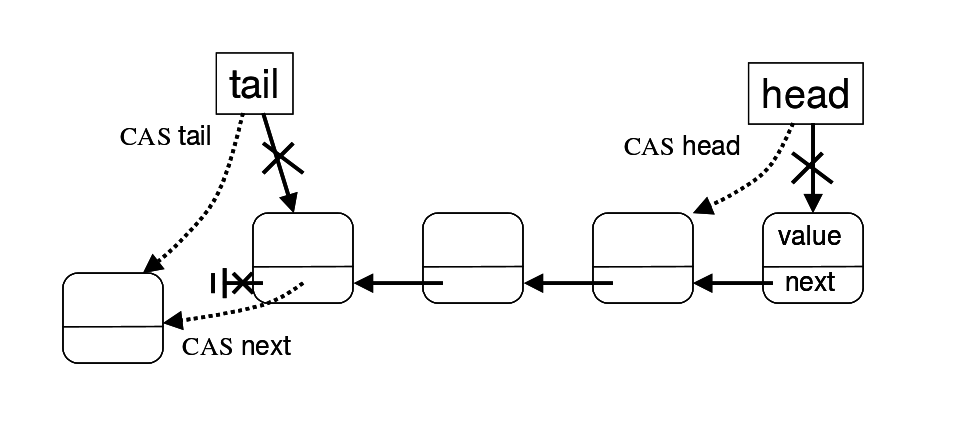
\includegraphics[scale=0.4]{msqueue_struct.png}
\caption{ Η δομή της συνδεδεμένης λίστας για την \textlatin{Michael Scott} υλοποίηση}
\end{figure}


Αντίθετα, για να αφαιρέσουμε κόμβο από την ουρά, αρκεί ένα \textlatin{C-A-S}  για να ενημερωθεί η τιμή του \textlatin{Head}.

%κωδικας για enq-deq??

Επειδή ανά πάσα στιγμή, κατά τη διάρκεια της εκτέλεσης ενός \textlatin{thread}, οι μεταβλητές \textlatin{Head} και \textlatin{Tail} μπορούν να αλλάξουν τιμή, πολλές φορές τα \textlatin{atomic operations} αποτυγχάνουν και η εκτέλεση ξεκινάει από την αρχή : διάβασμα του νέου \textlatin{Head/Tail} και προσπάθεια αλλαγής του με ατομικό τρόπο. Επίσης, επειδή για να έχουμε επιτυχημένο \textlatin{enqueue}, πρέπει να είναι επιτυχημένα και τα δύο \textlatin{CAS} που απαιτούνται, είναι πιθανόν ο κόμβος να προστεθεί στην ουρά χωρίς όμως να αλλάξει η τιμή του \textlatin{Tail}, δηλαδή να \textlatin{Tail} να μη δείχνει πλέον στο τελευταίο κόμβο. Για το λόγο αυτό, τόσο στο \textlatin{enqueue} όσο και sto \textlatin{dequeue}, γίνεται έλεγχος και διόρθωση του δείκτη \textlatin{Tail}.

Ένα από τα προβλήματα που προκύπτει κατά την υλοποίηση αυτού του αλγορίθμου, αλλά και γενικά σε μεθόδους που χρησιμοποιούν \textlatin{C-A-S} για συγχρονισμό , είναι το λεγόμενο ABA πρόβλημα. Συνοπτικά, το πρόβλημα περιγράφεται από το εξής σενάριο: Μια διεργασία διαβάσει τη τιμή Α από μια θέση μνήμης και στη συνέχεια  δέχεται μια καθυστέρηση. Στο ενδιάμεσο, μια άλλη διεργασία γράφει Β στην ίδια θέση μνήμης και στη συνέχεια την επαναφέρει ξανά σε κατάσταση Α. Η πρώτη διεργασία θα δει τη θέση μνήμης σε κατάσταση Α και το \textlatin{C-A-S} θα επιτύχει , χωρίς να έχει επίγνωση ότι η κατάσταση της μεταβλητής άλλαξε στο ενδιάμεσο. To πρόβλημα αυτό σχετίζεται με τη έλλειψη \textlatin{garbage collector} ή άλλου κατάλληλου μηχανισμού που εξασφαλίζει ότι δε μπορούμε να απελευθερώσουμε θέσεις μνήμης στις οποίες υπάρχει ακόμα κάποιο \textlatin{reference} .

Για να λύσουμε αυτό το πρόβλημα επιλέξαμε να χρησιμοποιήσουμε \textlatin{modifications counters} για κάθε \textlatin{pointer} που μας ενδιαφέρει, τους οποίους αυξάνουμε σε κάθε επιτυχημένο \textlatin{C-A-S}. To \textlatin{atomic operation} τώρα δε γίνεται μεμονωμένα στον δείκτη άλλα στο ζεύγος <δείκτης,\textlatin{modification counter}> το οποίο το μεταχειριζόμαστε σαν ενιαία μεταβλητή. Έτσι είμαστε αναγκασμένοι να κάνουμε τις αλλαγές στους δείκτες με μη παραδοσιακό τρόπο, σαν τμήμα μιας μεταβλητής, χρησιμοποιώντας εντολές για \textlatin{bit shifting}. Εναλλακτικά, στη βιβλιογραφία υπάρχουν άλλοι τρόποι για να λυθεί το ABA \textlatin{problem}, όπως για παράδειγμα η χρήση \textlatin{reference counters} που δεν απαιτεί τη συνένωση \textlatin{pointer} και \textlatin{counter}.

Το αποτέλεσμα είναι μια \textlatin{lock-free} υλοποίηση, που δεν απαιτεί κεντρικό κλείδωμα της δομής, αφήνει τα \textlatin{threads} να προχωρούν όλα μαζί και η επίδοση είναι ανεπηρέαστη από τυχαίες  καθυστερήσεις που μπορεί να δεχθεί κάποιο \textlatin{thread}. Εμφανίζει έτσι βελτιωμένη επίδοση σε σχέση με τη \textlatin{global-lock} υλοποίηση , ειδικά σε περιπτώσεις που τα \textlatin{threads} είναι περισσότερα από τα διαθέσιμα \textlatin{cores}.

%ίσως γραφική για msqueue

%lock-freeness/ορθότητα?


Ένα από τα μειονεκτήματα των \textlatin{lock-free} υλοποιήσεων είναι ότι κάθε φορά που ένα \textlatin{atomic operation} αποτυγχάνει, η εκτέλεση ξεκινάει από την αρχή. Πέρα από αυτό , τα ίδια τα \textlatin{atomic operations} εισάγουν καθυστέρηση, αφού απαιτούν συγχρονισμό στη μνήμη. Ειδικά στη περίπτωση αυτή, που απαιτούνται 2 επιτυχή \textlatin{atomic operations} για να ολοκληρωθεί το \textlatin{enqueue}, συμβαίνει συχνά κάποιο \textlatin{thread} να επαναλαμβάνει την εκτέλεση του ξανά και ξανά μέχρι να γίνει σωστά. Για το λόγο αυτό θα θέλαμε όσο γίνεται να  μειώσουμε τα σημεία συγχρονισμού, δηλαδή τα σημεία στα οποία γίνεται \textlatin{atomic operation}.

Μια λύση σε αυτό το πρόβλημα δίνει η επόμενη υλοποίηση που δοκιμάσαμε, από τους \textlatin{Ladan-Mozes} και \textlatin{Shavit} \cite{optimistic}. H υλοποίηση αυτή ακολουθεί μια \textlatin{optimistic} λογική(γι’ αυτό και θα αναφερόμαστε σε αυτή και σαν \textlatin{optimistic queue}) , με την έννοια ότι λειτουργεί γρήγορα με βάση την ευνοϊκή περίπτωση που δεν υπάρχει κάποιο \textlatin{conflict} και αφήνει τα χρονοβόρα operations μόνο για τη περίπτωση που παρατηρήθηκε ασυνέπεια στη δομή. Συγκεκριμένα, ένα από τα δύο \textlatin{C-A-S} κατά την \textlatin{enqueue} αντικαθίσταται  με απλό \textlatin{local store}, και στην συνέχεια φροντίζει να διορθώσει τη δομή με \textlatin{C-A-S} αν δεν είναι πλέον συνεπής.

Πρακτικά, η συνδεδεμένη λίστα αλλάζει φορά, με τους δείκτες να δείχνουν από το Tail προς το Head. Έτσι, αρκεί ένα C-A-S στο Tail ώστε να δείχνει στον καινούργιο κόμβο για να ολοκληρωθεί επιτυχώς ένα enqueue. Βέβαια, για να μπορούμε να έχουμε πρόσβαση στους κόμβου από το Head όταν κάνουμε dequeue, χρειαζόμαστε και δείκτες κατά την αντίθετη φορά, όπως φαίνεται και στο παρακάτω σχήμα.

%figure 2 apo optimistic paper
\begin{figure}
 \centering
  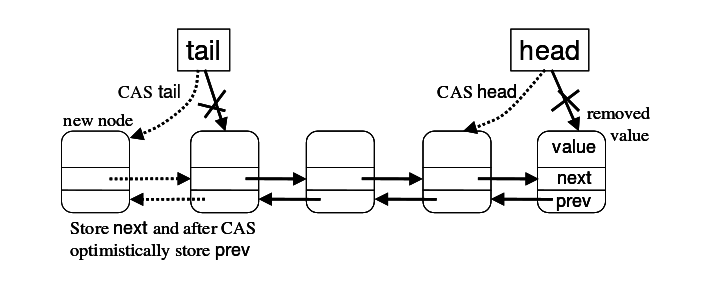
\includegraphics[scale=0.6]{optimistic_struct.png}
 \caption{ Η δομή της διπλά συνδεδεμένης λίστας για την \textlatin{Optimistic} υλοποίηση}
\end{figure}

\subsection{\textlatin{optimistic queue}}

Οι δείκτες και στις δύο κατευθύνσεις μεταβάλλονται με απλά \textlatin{stores}, χωρίς συγχρονισμό. Αυτό εμπεριέχει τον κίνδυνο οι δείκτες κατά την κατεύθυνση \textlatin{prev} να μην είναι συνεπείς. Για το λόγο αυτό, μόλις διαπιστωθεί ασυνέπεια, καλείται κατάλληλη συνάρτηση( \textlatin{FixList}) που διατρέχει τη λίστα και διορθώνει τους \textlatin{pointers}. Το πόσο συχνά όμως συμβαίνουν ασυνεπείς, έχει να κάνει με τις ατομικές καθυστερήσεις που μπορεί να δεχθεί ένα \textlatin{thread} και όχι με τη συμφόρηση. Έτσι, ο αριθμός των κλήσεων στην \textlatin{FixList} παραμένει χαμηλός, ακόμα και όταν ο αριθμός των παράλληλων \textlatin{threads} μεγαλώνει.

Για να αποφύγει το ABA πρόβλημα αλλά και να εντοπίζει ασυνέπειες στους pointers, αυτή η υλοποίηση χρησιμοποιεί επίσης \textlatin{modification counters} που ενσωματώνονται στους δείκτες και αυξάνονται κατά ένα σε κάθε επιτυχημένη \textlatin{C-A-S}.

H διαδικασία της εισαγωγής κόμβου στη λίστα περιλαμβάνει 3 βήματα:
1) Αλλαγή του \textlatin{next pointer} στον προς εισαγωγή κόμβο
2) \textlatin{C-A-S} στο \textlatin{Tail} ώστε να δείχνει στον νέο κόμβο
3) Αλλαγή του \textlatin{prev pointer} του επόμενου κόμβου

Κάθε φορά οι αλλαγές στους \textlatin{pointers} γίνονται μαζί με τους αντίστοιχους \textlatin{modification counters}.

Κάποιο \textlatin{thread} ενδέχεται να δεχθεί καθυστέρηση ανάμεσα στο βήμα 2 και 3, με αποτέλεσμα να μπουν στην  ουρά και άλλοι κόμβοι και έτσι ο \textlatin{prev pointer} να μην δείχνει όντως τον προηγούμενο κόμβο. Επειδή όμως, κάθε  φορά που κάποιος κόμβος εισέρχεται στη λίστα(επιτυχημένο \textlatin{C-A-S}) αυξάνεται κατά ένα ο \textlatin{modification counter} που γράφεται στον κόμβο, προκύπτει ότι \textlatin{pointers} γειτονικών κόμβων στη λίστα θα έχουν διαδοχικούς \textlatin{modification counters}. Έτσι κατά το \textlatin{dequeue}, αν βρεθεί κόμβος που o \textlatin{prev pointer} του δεν έχει σωστό \textlatin{modification counter}, καλείται η \textlatin{FixList} που διατρέχει όλη τη λίστα και διορθώνει τους \textlatin{prev pointers}.

Σημειώνουμε ότι πρέπει να υπάρχει ειδική φροντίδα ώστε να υπάρχει πάντα ένας \textlatin{dummy node} στη λίστα και ο \textlatin{Tail}  να μην τον ξεπερνάει.

Το παρακάτω διάγραμμα συγκρίνει τα \textlatin{C-A-S operations}( επιτυχημένα και μη) που χρειάστηκαν για να εκτελεστούν 1 εκατομμύριο ζεύγη \textlatin{enqueue/dequeue} για τις δύο αυτές εκδόσεις. Παρατηρούμε ότι η \textlatin{optimistic} υλοποίηση πραγματοποιεί αυτό που υπόσχεται , δηλαδή απαιτεί λιγότερα \textlatin{C-A-S}  και έχει συνολικά λιγότερα χρονοβόρα, αποτυχημένα \textlatin{atomic operations} καθώς ο αριθμός των παράλληλων \textlatin{threads} μεγαλώνει.

%διαγραμμα για failed CAS
\begin{figure}
 \centering
  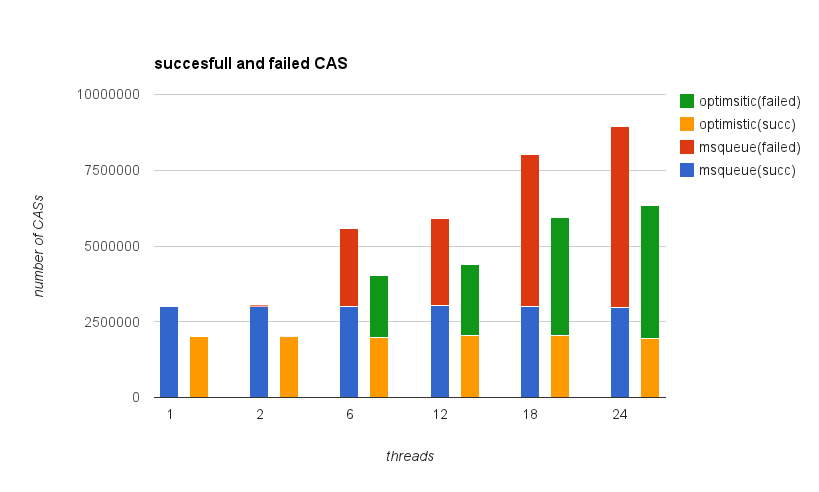
\includegraphics[scale=0.5]{failed_cas.png}
\caption{Τα συνολικά επιτυχημένα και αποτυχημένα\textlatin{C-A-S} για τις δύο υλοποιήσεις}
\end{figure}

\subsection{\textlatin{Flat Combining}}

Οι δύο προηγούμενες υλοποιήσεις ακολούθησαν \textlatin{fine grained} λογική, όπου κάθε \textlatin{thread} έχει πρόσβαση στη δομή και προσπαθούν να βελτιώσουν την απόδοση μέσα από τον υψηλό παραλληλισμό. Δίνοντας την ευκαιρία σε περισότερα threads να εκτελούν τα operations τους στη δομή, οδηγεί σε καλύτερη επίδοση από το \textlatin{locking} υλοποιήσεις που μπλοκάρουν την πρόδο κάποιον \textlatin{threads}. Στη συνέχεια παρουσιάζεται η βασική ιδέα του \textlatin{flat combining}, ενός τρόπου προγραμματισμού από τους \textlatin{Hendler, Incze} και \textlatin{Shavit} \cite{flat_combining}, που αντιτίθεται στη παραπάνω λογική. 

Συγκεκριμένα, οι συγγραφείς υποστηρίζουν ότι το σημείο στο οποίο το κόστος του συγχρονισμού πολλών \textlatin{threads} υπερβαίνει το κέρδος από την υψηλή παραλληλία, εμφανίζεται σε πολύ μικρότερα επίπεδα παραλληλίας απότι θα περίμενε κανείς. Το \textlatin{flat combining} στηρίζεται σε έναν τρόπο συγχρονισμού όπου ένα \textlatin{thread}, κλειδώνει τη δομή με εξαιρετικά χαμηλό κόστος, μαθαίνει όλα τα τρέχοντα \textlatin{operations} που προσπαθούν να εκτελεστούν στη δομή από τα υπόλοιπα \textlatin{treads} και εκτελεί αυτό συγκεντρωτικά τα \textlatin{operations} στη θέση τους. Το αποτέλεσμα είναι μια υλοποίηση με χαμηλό κόστος συγχρονισμού αλλά και καλύτερη συμπεριφορά ως προς την \textlatin{cache}, τα οφέλη της οποίας ξεπερνούν το κόστος του κεντρικού κλειδώματος και του μειωμένου παραλληλισμού.

To \textlatin{flat combining} αποτελεί ένα \textlatin{layer} που μπορεί να τοποθετηθεί πάνω από μια \textlatin{sequential} δομή και λειτουργεί σε βασικές γραμμές ως εξής:
1) κάθε \textlatin{thread} γράφει τη λειτουργία που θέλει να εκτελέσει και τις παραμέτρους της σε ένα \textlatin{public record} που ανήκει σε αυτό το \textlatin{thread}. Τα \textlatin{public records} μπορούν να είναι οργανωμένα σε πίνακα, για γρήγορο \textlatin{read/write} ή σε λίστα με μήκος που μεταβάλεται δυναμικά ανάλογα με το πλήθος των \textlatin{active threads}.
2) κάθε \textlatin{thread} προσπαθεί μία φορά , με ατομικό τρόπο, να πάρει το \textlatin{lock} της δομής. Αν διαπιστώσει ότι η δομή είναι κλειδωμένη, περιμένει διαβάζοντας το \textlatin{public record} του μέχρι να του έρθει η απάντηση για το \textlatin{operation} που δήλωσε ότι θέλει να εκτελέσει.
3) αν πάρει το \textlatin{lock}, το \textlatin{thread} θεωρείται ως ο νέος \textlatin{combiner} και αναλαμβάνει αυτό να εκτελέσει τα \textlatin{requests} των υπολοίπων. Διατρέχει όλα τα \textlatin{public records}, εκτελεί ένα ένα τα \textlatin{request} και επιστρέφει τα αποτελέσματα στα κατάλληλα \textlatin{public records}. Τέλος ελευθερώνει το \textlatin{lock}.

%isws kanena sxhmataki san ayto poy exei sto paper

Από τον τρόπο που λειτουργεί το \textlatin{flat combining} προκύπτουν κάποια βασικά πλεονεκτήματα:
1) επειδή μόνο ο \textlatin{combiner} έχει πρόσβαση στη δομή, τα \textlatin{operations} μπορούν να γίνουν με τον καλύτερο δυνατό \textlatin{sequential} αλγόριθμο, χωρίς να μας απασχολούν θέματα που αφορούν τη παραλληλία και τον συγχρονισμό. Αυτό επιτρέπει να υλοποιήσουμε παράλληλες δομές, όπως \textlatin{pairing heaps}, που δεν μπορούν εύκολα να συγχρονιστούν με \textlatin{fine-grained} τρόπο, χρησιμιποιώντας \textlatin{flat combining} πάνω από ήδη υπάρχουσες \textlatin{sequential} δομές.
2) σε κάποιε δομές, ο \textlatin{combiner} μπορεί να χρησιμοποιεί κάποιον έξυπνο τρόπο για να ομαδοποιεί τα \textlatin{request} και έτσι η πρόσβαση στη δομή να είνα ακόμα πιο γρήγορη και αποδοτική. Για παράδειγμα, σε \textlatin{concurrent stacks}, ο \textlatin{combiner} μπορεί να κάνει \textlatin{ellimination} ανάμεσα σε ένα \textlatin{enqueue} και ένα \textlatin{dequeue} που προσπαθούν να εκτελεστούν στη δομή. Στις ουρές που υλοποιήσαμε χρησιμοποιήσαμε \textlatin{fat nodes} που ομαδοποιούν τα στοιχεία , όπως θα εξηγήσουμε αργότερα.
3) Ο συγκεντρωτικός τρόπος με τον οποίο γίνεται το \textlatin{access} στη δομή, μπορεί να οδηγήσει σε καλύτερη αξιοποίηση τη \textlatin{cache}.
4) χρησιμοποιώντας \textlatin{global lock} είναι πιο εύκολος ο προγραμματισμός της δομής και ο εντοπισμός λαθών.

Σημαντικό είναι επίσης ότι το \textlatin{flat combinbing} αποτελεί ένα αφαιρετικό επίπεδο που εξασφαλίζει συγχρονισμό και μπορεί να χρησιμοποιηθεί αυτούσιο  πάνω από διαφορετικές δομές. Βέβαια, δεν επωφελούνται όλες οι δομές από το \textlatin{flat combing}. Για παράδειγμα, αν σε ένα \textlatin{search tree} ένα \textlatin{operation} έχει κόστος Θ(\textlatin{logn}), χρησιμοποιώντας \textlatin{flat combining, k} operations απαιτούν Θ(\textlatin{klogn}) χρόνο, ένω εν γένει θα μπορουσαμε να έχουμε παράλληλα \textlatin{threads} που εκτελούν ανεξάρτητα τα \textlatin{operations} σε δίαφορα σημεία του δέντρου σε Θ(\textlatin{logn}) χρόνο συνολικά.

Συγκεκριμένα οι ουρές, φαίνονται πως ευνοούνται από το \textlatin{flat combining}, δεδομένου ότι ήδη έχουν μειωμένη παραλληλία ( τα \textlatin{access points} είναι μόνο δύο). Στην υλοποίηση μας οργανώσαμε τα \textlatin{public records} σε πίνακα και χρησιμοποιήσαμε τη λογική των \textlatin{fat nodes}, όπου κάθε node χωράει 16 στοιχεία. Έτσι για κάθε 16 \textlatin{enqueues}, θα χρειαστεί να προσθέσουμε μόνο ένα κόμβο στην ουρά και θα κάνουμε μόνο μια μετακίνηση στον \textlatin{pointer Tail}. Επίσης χρησιμοποιήσαμε δύο ανεξάρτητα \textlatin{instances} του \textlatin{flat combining}, ένα που αφορά τα \textlatin{enqueues} και ένα για τα \textlatin{dequeues}, ώστε να αξιοποιήσουμε το μέγιστο δυνατό παραλληλισμό της δομής. 




\newpage
\small
\noindent
\selectlanguage{greek}  % mine
% mine -- maybe more text about copyrights, etc here.
\copyright \hspace{1em}(Εισάγετε έτος έκδοσης) Εθνικό Μετσόβιο Πολυτεχνείο.
\selectlanguage{english}  % mine
\textlatin{All rights reserved.}

\newpage
\selectlanguage{greek}  % mine
\printindex  % mine -- do you use one?
\nocite{*}
\bibliographystyle{babplain-fl}  %mine -- for name-surname order
\bibliography{references}  % mine -- the references.bib file
\end{document}
